\documentclass[../main.tex]{subfiles}

\begin{document}

\section{Introduction}
\label{sec:intro}

% % Key audiences to reach:
% Mathematicians \& continuum modellers new to batteries
% DFT users: a) DFT developers, b) Applying DFT to models on other length scales, c) Atomistic models other than DFT: Monte carlo, MD, etc.
% Battery modellers at other scales: Continuum (both) and control modellers (atomistic $\to$ control) is made in the anodes section already.
% Other battery experts: a)Battery experimentalists in materials development – most of the other Faraday projects, b) Theorists in materials discovery, c) Electrochemical engineers – Greg, Dave Howey etc.
% Scientists new to batteries (the ``battery curious'')

% % Who to highlight where:
% Introduction: focuses on introducing newcomers to batteries and/or atomistic modellers (e.g. new PhD students, postdocs switching fields, etc.), preach to DFT users (a-c), and give one/two sentences link with experiment and continuum models. We should provide a breakdown of the review structure, highlighting there who we think might be interested in each of the main sections.
% Main text: Audience will necessarily differ in each subsection but we can clearly signpost in the introduction which part is relevant to whom so that the right people can find the relevant bits. Important, as the majority of readers will not read the whole review.
% Outlook: mirrors the introduction in terms of audience and will be broken down into 5-6 bullets as outstanding challenges. One of these will be the link to the different continuum and control models. Link to experiment might need to be a separate point.

% *******************************************************************************

Lithium-ion (Li-ion) batteries (LiBs) were first commercialised by Sony in 1991. \cite{zeng2019commercialization} They are ubiquitous in portable electronic devices, are emerging in hybrid and all-electric vehicles, \cite{Goodenough2010} and are starting to play a role in large-scale stationary storage. \cite{kubiak2017calendar} Despite over 30 years of commercialisation and longer for development, not all factors dictating their capacity, performance, safety, and longevity are completely understood. The complexity of battery systems makes it time consuming and impractical to directly measure all of their physical attributes. The grand challenge is to construct a multiscale model, incorporating inputs across length- and time-scales that can not only describe, but also predict, changes in behaviour.

To build a truly predictive modelling framework, a physical underpinning to battery models is required, incorporating physically correct descriptions of thermodynamic and kinetic battery behaviour. With sufficient accuracy built in, these models can provide insights on difficult-to-measure internal states, such as degree of Li intercalation and local electrolyte and ionic concentrations, as determined by the nanostructure of the materials used. By contrast, empirical models, which fit a curve to experimental data, are widely used in battery research, but have only a limited physical basis or, in some cases, no physical basis at all. For example, equivalent circuit models, which are widely used in industry, cannot be relied upon to predict battery behaviour over several charge-discharge cycles.

Physics-based continuum models attempt to describe the behaviour of whole cells, for example the widely used Doyle-Fuller-Newman (DFN) model. \cite{doyle1993modeling, fuller1994simulation, Fuller1994a,Doyle1995,Newman2004} These models need to use drastic simplifications to enable them to run in real time, but their accuracy can be greatly improved by adopting parameters measured using more detailed, microscopic simulations. Atomistic models are key to building truly physics-based models and form the foundation of the multiscale modelling chain, leading to more robust and predictive models.
 
Atomistic models can also be applied to fundamental research questions with high predictive accuracy. For example, they can be used to predict new behaviour not currently accessible by experiment, for reasons of cost, safety, or throughput. They can be used to optimise experimental design and use resources more efficiently, determining whether particular experiments are even worth performing and also provide unique insights into the behaviour of materials that may not even be accessible, or are impractical to obtain, by experimental probes. Atomistic models are useful for quantifying and evaluating trends in experimental data, explaining structure-property relationships and informing materials design strategies and libraries.

% METHODS SUMMARY
The family of atomistic models itself represents a range of different length- and time-scales, from the level of electronic structure calculations through conventional and linear-scaling Density Functional Theory (DFT), to \textit{ab initio} Molecular dynamics (MD) and on to longer length scale models, such as classical MD, Monte Carlo (MC), and kinetic Monte Carlo (kMC) calculations, which are parameterised by force field potentials or \textit{ab initio} data. These techniques, along with recent method developments and battery-specific observable properties, are summarised in the methods section of this review, section~\ref{sec:methods}. Specific applications to anodes, liquid and solid electrolytes, and cathodes are broken down in the following sections. Links between different methodologies are emphasised and this review may thus be of particular interest to those looking, for example, to link DFT calculations to MC calculations, or apply linear-scaling DFT to MD, bridging possible gaps in nomenclature at different length scales. Atomistic models linking to \textit{ab initio} calculations are summarised by \citeauthor{VanderVen2020} \cite{VanderVen2020}; also noteworthy in this area is a review by \citeauthor{Shi_2016},\cite{Shi_2016} and an older review by \citeauthor{franco2013multiscale}.\cite{franco2013multiscale} A recent review of method development in the area of hybrid quantum-continuum solvation models is presented by \citeauthor{Herbert2021}.\cite{Herbert2021}

\begin{figure}
    \centering
    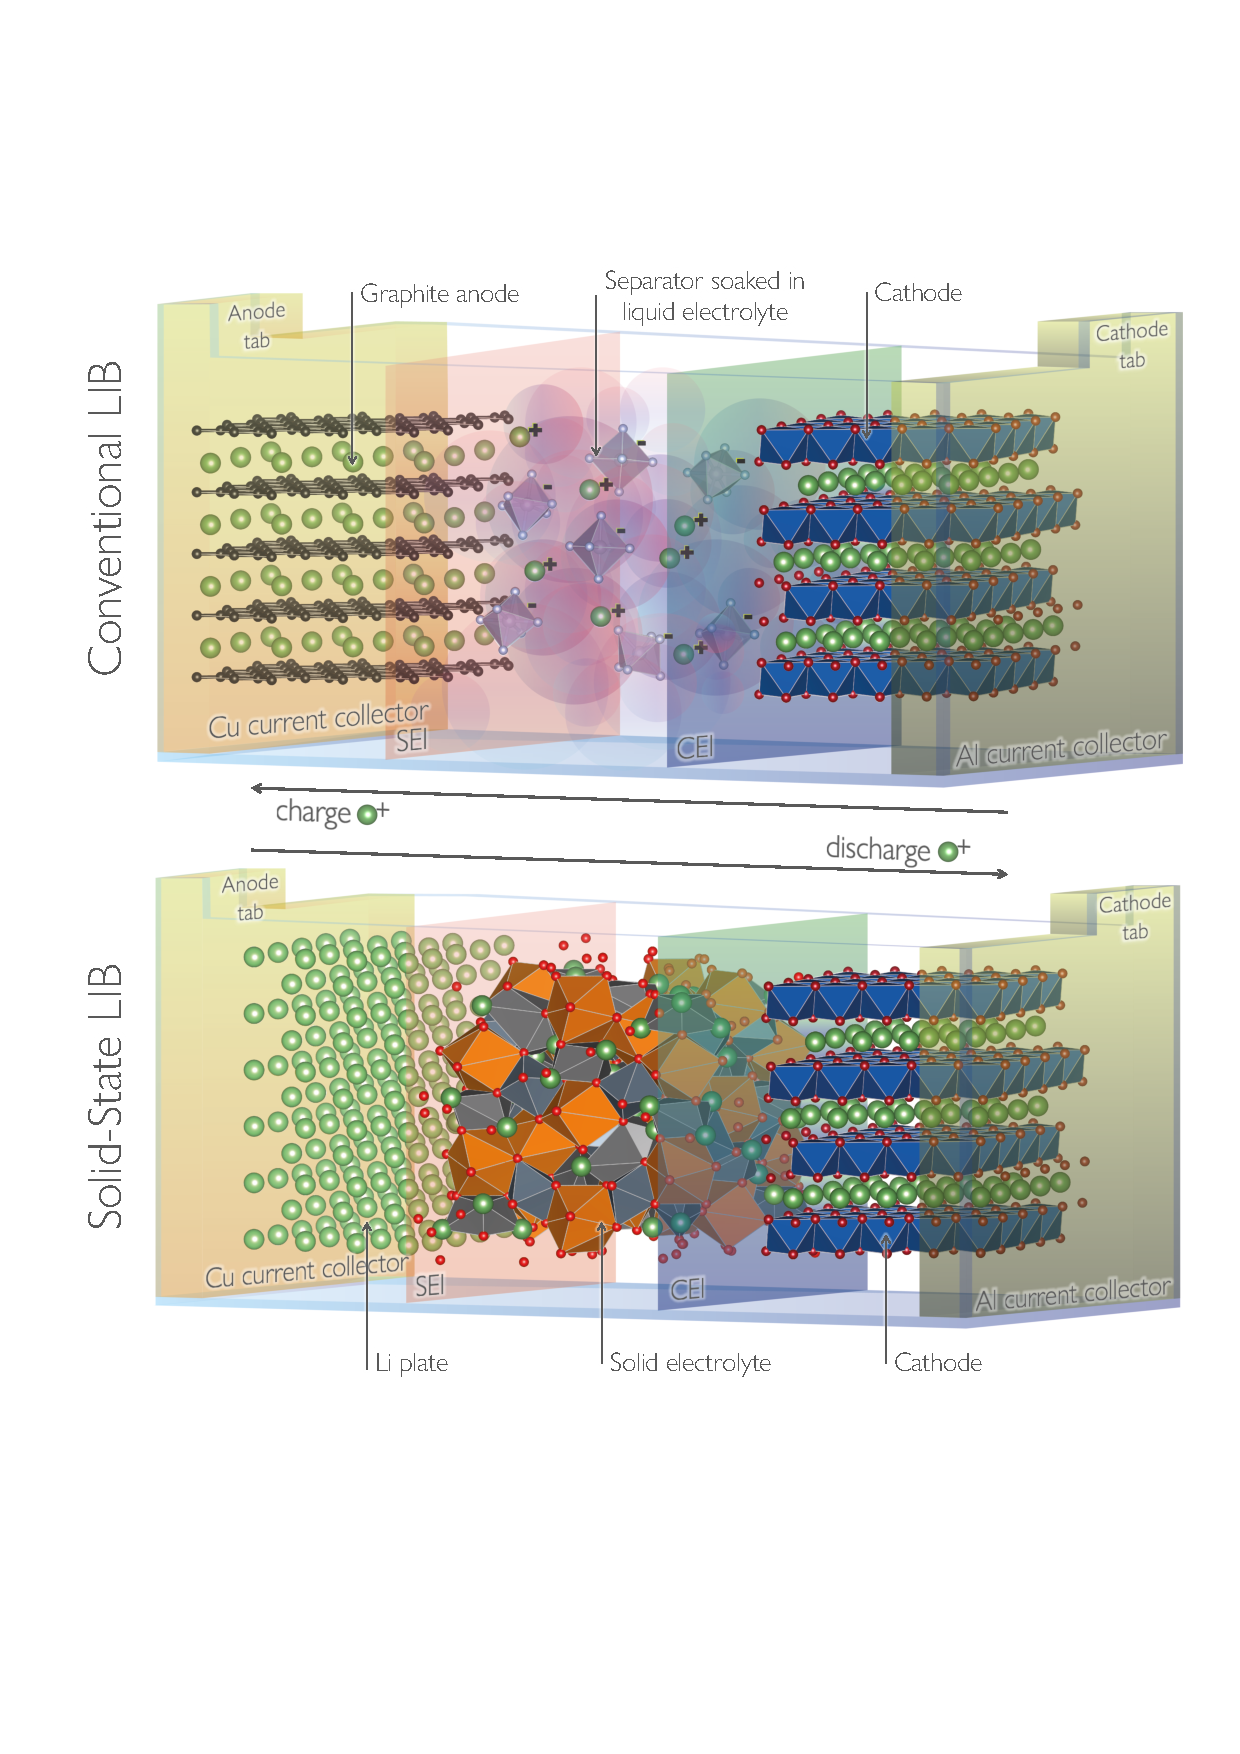
\includegraphics[scale=0.6]{figures/battery_design.pdf}
    \caption{A schematic of a single cell of a conventional, liquid-based lithium-ion battery (LiB) and a solid-state LiB. The conventional LiB comprises an anode composed of a Cu current collector and an active anode material (graphite), a separator soaked in an organic electrolyte, and a cathode composed of a Al current collector and an active cathode material, for example, LiCo$_2$, as shown here. The solid-state LiB comprises a similar cathode, a solid electrolyte, and an anode composed of a Li-ion plate and Cu current collector. The anode-electrolyte interphase (SEI) and cathode-electrolyte interphase (CEI) for both LiBs are represented as pink and blue transparent layers, respectively. The tabs are shown protruding from the top of the current collectors. Both LiB cells show all components as fully lithiated, with directional Li$^+$ movement during (dis)charge indicated with arrows.}
    \label{fig:battery_schematic}
\end{figure}

The review covers mechanisms in both the conventional liquid electrolyte based and solid-state based LiB, as shown schematically in Figure~\ref{fig:battery_schematic}. In a single cell of a conventional LiB, as shown here, the anode, or negative electrode, comprises a copper current collector and the primary active material is graphite in the vast majority of commercial LiBs. The two electrodes are divided by a separator soaked in an organic electrolyte, which is usually a mixture of carbonates with dissolved LiPF$_{6}$ salt. The cathode, or the positive electrode, has an aluminium current collector. Various different types of cathode material are utilised in commercial LiBs, with the example shown here being the classic ``rocking-chair'' battery with a LiCO$_{2}$ cathode.\cite{Scrosati_1992} When the cell is assembled, the cathode starts fully lithiated and the anode is completely delithiated. On the first cell charge cycle (also known as the formation cycle) lithium is removed from the cathode and the anode becomes filled with lithium while the solid electrolyte interphase (SEI) and cathode electrolyte interphase (CEI) are formed. While Figure~\ref{fig:battery_schematic} shows both electrodes in a fully lithiated state, Li is transferred between the electrodes reversibly during (dis)charging, therefore allowing this system to be rechargeable.

Although not yet commercialised, solid-state LiBs are a promising future alternative to conventional liquid electrolyte LiBs. Their anode, or negative electrode, comprises a copper current collector and either a a metallic lithium plate (Li-metal), as shown in Figure~\ref{fig:battery_schematic}, or less commonly a graphite-based material (Li-ion). As there is no liquid, there is no longer a need for separators, with the two electrodes being separated by the solid electrolyte material, shown here with Li$_7$La$_3$Zr$_2$O$_2$ (LLZO). The cathode, or positive electrode, has an aluminium current collector and, as with the conventional LiB, can accommodate various cathode materials, such as LiCo$_2$. The interfacial regions between the electrodes and the solid electrolyte are known as the solid-solid interphase, or anode/cathode-solid interphase. Figure~\ref{fig:battery_schematic} shows both electrodes in a fully lithiated state; however, the Li is transferred between the electrodes reversibly, as in conventional LiBs.

% ANODES SUMMARY
The anodes section, section~\ref{sec:anodes}, heavily focuses on graphite, which is still the predominant anode material in Li-ion cells. The section describes atomistic modelling of bulk graphite, graphite edges where initial Li-ion insertion occurs, and the Solid-Electrolyte Interphase (SEI). The bulk modelling discussion includes a direct comparison between experimental and theoretical thermodynamic parameters, such as the open circuit voltage (OCV) and entropy, which will also be of interest to battery control modellers. Kinetic predictions are made and linked to DFT predictions of the influence of graphite edge morphology on surface states, which may be of interest to those working on battery material development and discovery. Recent work applying linear scaling DFT to complex interfaces will be of interest to those at the forefront of DFT method development, focusing on the boundary between atomistic and continuum modelling. Lastly, recent developments in silicides to boost anode gravimetric capacity, along with their associated challenges, are summarised in the outlook. Recent reviews in this area include \citeauthor{asenbauer_success_2020} \cite{asenbauer_success_2020}, summarising aspects of lithiation/delithiation mechanisms and morphological aspects in graphite and silicon oxide composites, and \citeauthor{ZHANG2021147} \cite{ZHANG2021147}, similar in scope but providing a more \textit{ab initio} focus. Here, our review here covers graphite structure and lithiation/delithiation mechanisms, including surfaces and interfaces, which have tended to be neglected, although aspects of modelling the SEI have been reviewed by \citeauthor{Wang2018}. \cite{Wang2018}

% LIQUID ELECTROLYTES SUMMARY
The liquid electrolyte section, section~\ref{sec:Liquid_electrolytes}, has a strong focus on the development of atomistic models, both \textit{ab initio} and force field-based. This includes a pivotal discussion on the atomic interactions between the components and method development to study electrolytes via classical MD simulations. This will be of particular interest to those at the forefront of classical MD method development. Liquid electrolytes are known to be limited by narrow electrochemical windows, solvent toxicity, and material flammability/safety concerns. The latter parts of this section describe the atomistic modelling of the bulk structure and landscaping, Li-ion diffusion, solvation energies, and activity coefficients of liquid electrolytes, and the interfacial nanostructure relating to the interface with a solid electrode. These topics cover the major aspects for improving liquid electrolytes for use in a battery and research towards circumventing critical safety\cite{Shepherd_Siddiqui, Pfrang2017} and energy density\cite{Liu2019_e_den} limitations. The challenges and potential avenues for solving these issues are summarised in the outlook, including recent developments to resolve these within the liquid electrolyte family and alternative materials. Recent reviews in this area include \citeauthor{galinski2006ionic},\cite{galinski2006ionic} summarising the field of ionic liquids, \citeauthor{wang2020recent},\cite{wang2020recent} reviewing the recent progress in water in salts electrolytes, and \citeauthor{Logan2020},\cite{Logan2020} giving some recent developments in conventional electrolytes. Here, our review covers the continued development of interatomic potentials for liquid electrolytes and a description of the solid electrode-liquid electrolyte interface from the perspective of the liquid, which is not the conventional frame of reference.

% SOLID ELECTROLYTES SUMMARY
Solid electrolytes (SEs) are becoming an increasingly popular avenue of research, motivated by the rise of the electric vehicle (EV). \cite{Woods_2021} They have been proposed as an alternative to liquid electrolytes to resolve safety issues pertaining to the flammable organic liquid electrolytes that are currently used,\cite{Shepherd_Siddiqui, Pfrang2017} and also as a route to increased energy density\cite{Liu2019_e_den}. In the solid electrolyte section, section~\ref{sec:solid_electrolytes}, we review a selection of the promising candidate materials currently being investigated. Each material discussed has a different focus, highlighting a range of properties applicable to different SE materials. In this section, we focus on four material families, grouping them into sulfide and oxide based SEs. Sulfide based SEs typically have a high Li-ion conductivity and poor electrochemical stability against Li metal (the anode typically used in combination with SEs). \cite{Zhu2015, Zhang2019se_rev} Li$_{10}$GeP$_2$S$_{12}$ (LGPS) is reviewed, with a focus on how atomistic methods reveal the isotropic ion pathways, while Li$_6$PS$_5$\textit{X} based Li-argyrodites are focused towards the relationship between ionic conductivity and anion substitution, as well as atomistic predictions of occupied Li sites. Oxides typically have a higher electrochemical stability but still suffer from dendrite formation, amongst other issues.\cite{Zhu2015} LLZO is also reviewed, with a focus on how multiple atomistic methods have been applied to probe dendrite formation and ionic transport in the material. State-of-the-art models of interfaces in oxide nanocomposites are reviewed. Lastly, the challenges of the SEI are discussed and an outlook to future modelling of SEs is given. Related reviews in the area include \citeauthor{Zhang2018se_review}, \cite{Zhang2018se_review} summarising the future directions of solid-state batteries (SSBs), and \citeauthor{Gurung2019}, \cite{Gurung2019} highlighting the advances and challenges in SEs and SSBs. \citeauthor{Xiao2020interfacerev}\cite{Xiao2020interfacerev} and others\cite{Xu2018exp,Tateyama2019} provide a more specific review of the SEI. \citeauthor{Ceder2018} \cite{Ceder2018} outlines the principles that should be employed when modelling SEs. Here, our review discusses a broad range of SE properties, following the notion that these properties are applicable to range of materials.

% CATHODES SUMMARY
The cathodes section, section~\ref{sec:cathodes}, covers a range of different cathode materials used in a variety of Li-ion cells. This section describes atomistic modelling in the bulk, at the surfaces, and the Cathode-Electrolyte Interphase (CEI). In discussing bulk modelling, a comparison of the different cathode crystal structures, micro-structuring, and available diffusion pathways within the material are covered, as well as important properties, including redox and electronic properties, transition metal ordering, and vibrational and thermal properties. Use of \textit{First Principles} modelling techniques has been essential for investigating crystalline structure, so will be of great interest to those who utilise DFT in their research. Surface structures and morphologies of cathode particles can be difficult to determine using experimental methods alone, which is where \textit{ab initio} and potentials-based MD can provide vital insight. As with the SEI, linear scaling DFT has recently been applied to CEI, where discussions on CEI will be of interest to those doing state-of-the-art DFT method development. Related reviews in the area include \citeauthor{ma2018computer}, \cite{ma2018computer} summarising modelling Li-ion battery cathode materials, \citeauthor{yan2014review}, \cite{yan2014review} focusing on \textit{First Principles} calculations of cathode materials, and \citeauthor{wang2018reviving}, \cite{wang2018reviving} discussing closing the gap between theoretical and practical capacities in layered oxide cathode materials. Our review includes a discussion on the CEI, which has recently been reviewed by \citeauthor{maleki2019controllable}. \cite{maleki2019controllable} Here, our review covers thermal, electronic, dynamic, and structural properties for a range of prominent cathode materials in terms of both \textit{First Principles} and potential-based modelling, which have tended to be more isolated in other reviews.

Finally, we provide an outlook on the key remaining challenges for atomistic modelling of LiBs and promising future directions for resolving them.

\end{document}